%!TEX root = ../swiatlow_thesis.tex
\label{chapter:jet-reconstruction}


Jet reconstruction in ATLAS makes use of the algorithms described in~\ref{chapter:jets-and-substructure} to create 4-vectors and other observables usable for physics analysis. As previously discussed, a wide variety of algorithms, with various uses and benefits compared to others, are available in the literature. ATLAS most typically makes use of:

\begin{enumerate}
	\item \antikt with $R = 0.4$
	\item \antikt with $R = 0.6$
	\item \antikt with $R = 1.0$, using Trimming with $\Rsub = 0.3$, $\fcut = 5\%$
\end{enumerate}
%
Some analyses also make use of various \CAFat jets, with various forms of split-filtering or reclustered-mass-drop filtering \editnote{Cite these.}. The analyses presented in in this thesis utilize the first and third algorithms, and most of the discussion that follows will focus on various aspects of the reconstruction of these jets.

There are many more aspects to creating a jet than just choosing an algorithm, and this chapter covers the various aspects of jet reconstruction from inputs to calibrations and flavor identification. 

\section{Jet Inputs}


One of the most important decisions in constructing a jet is the decision of what to actually input to the jet algorithm-- i.e., the choice of what to cluster. Several inputs are available, summarized in Figure~\ref{fig:jet-reconstruction:making-jets}. 

%%%%%%%%%%%%%%%%

\begin{figure}
\centering
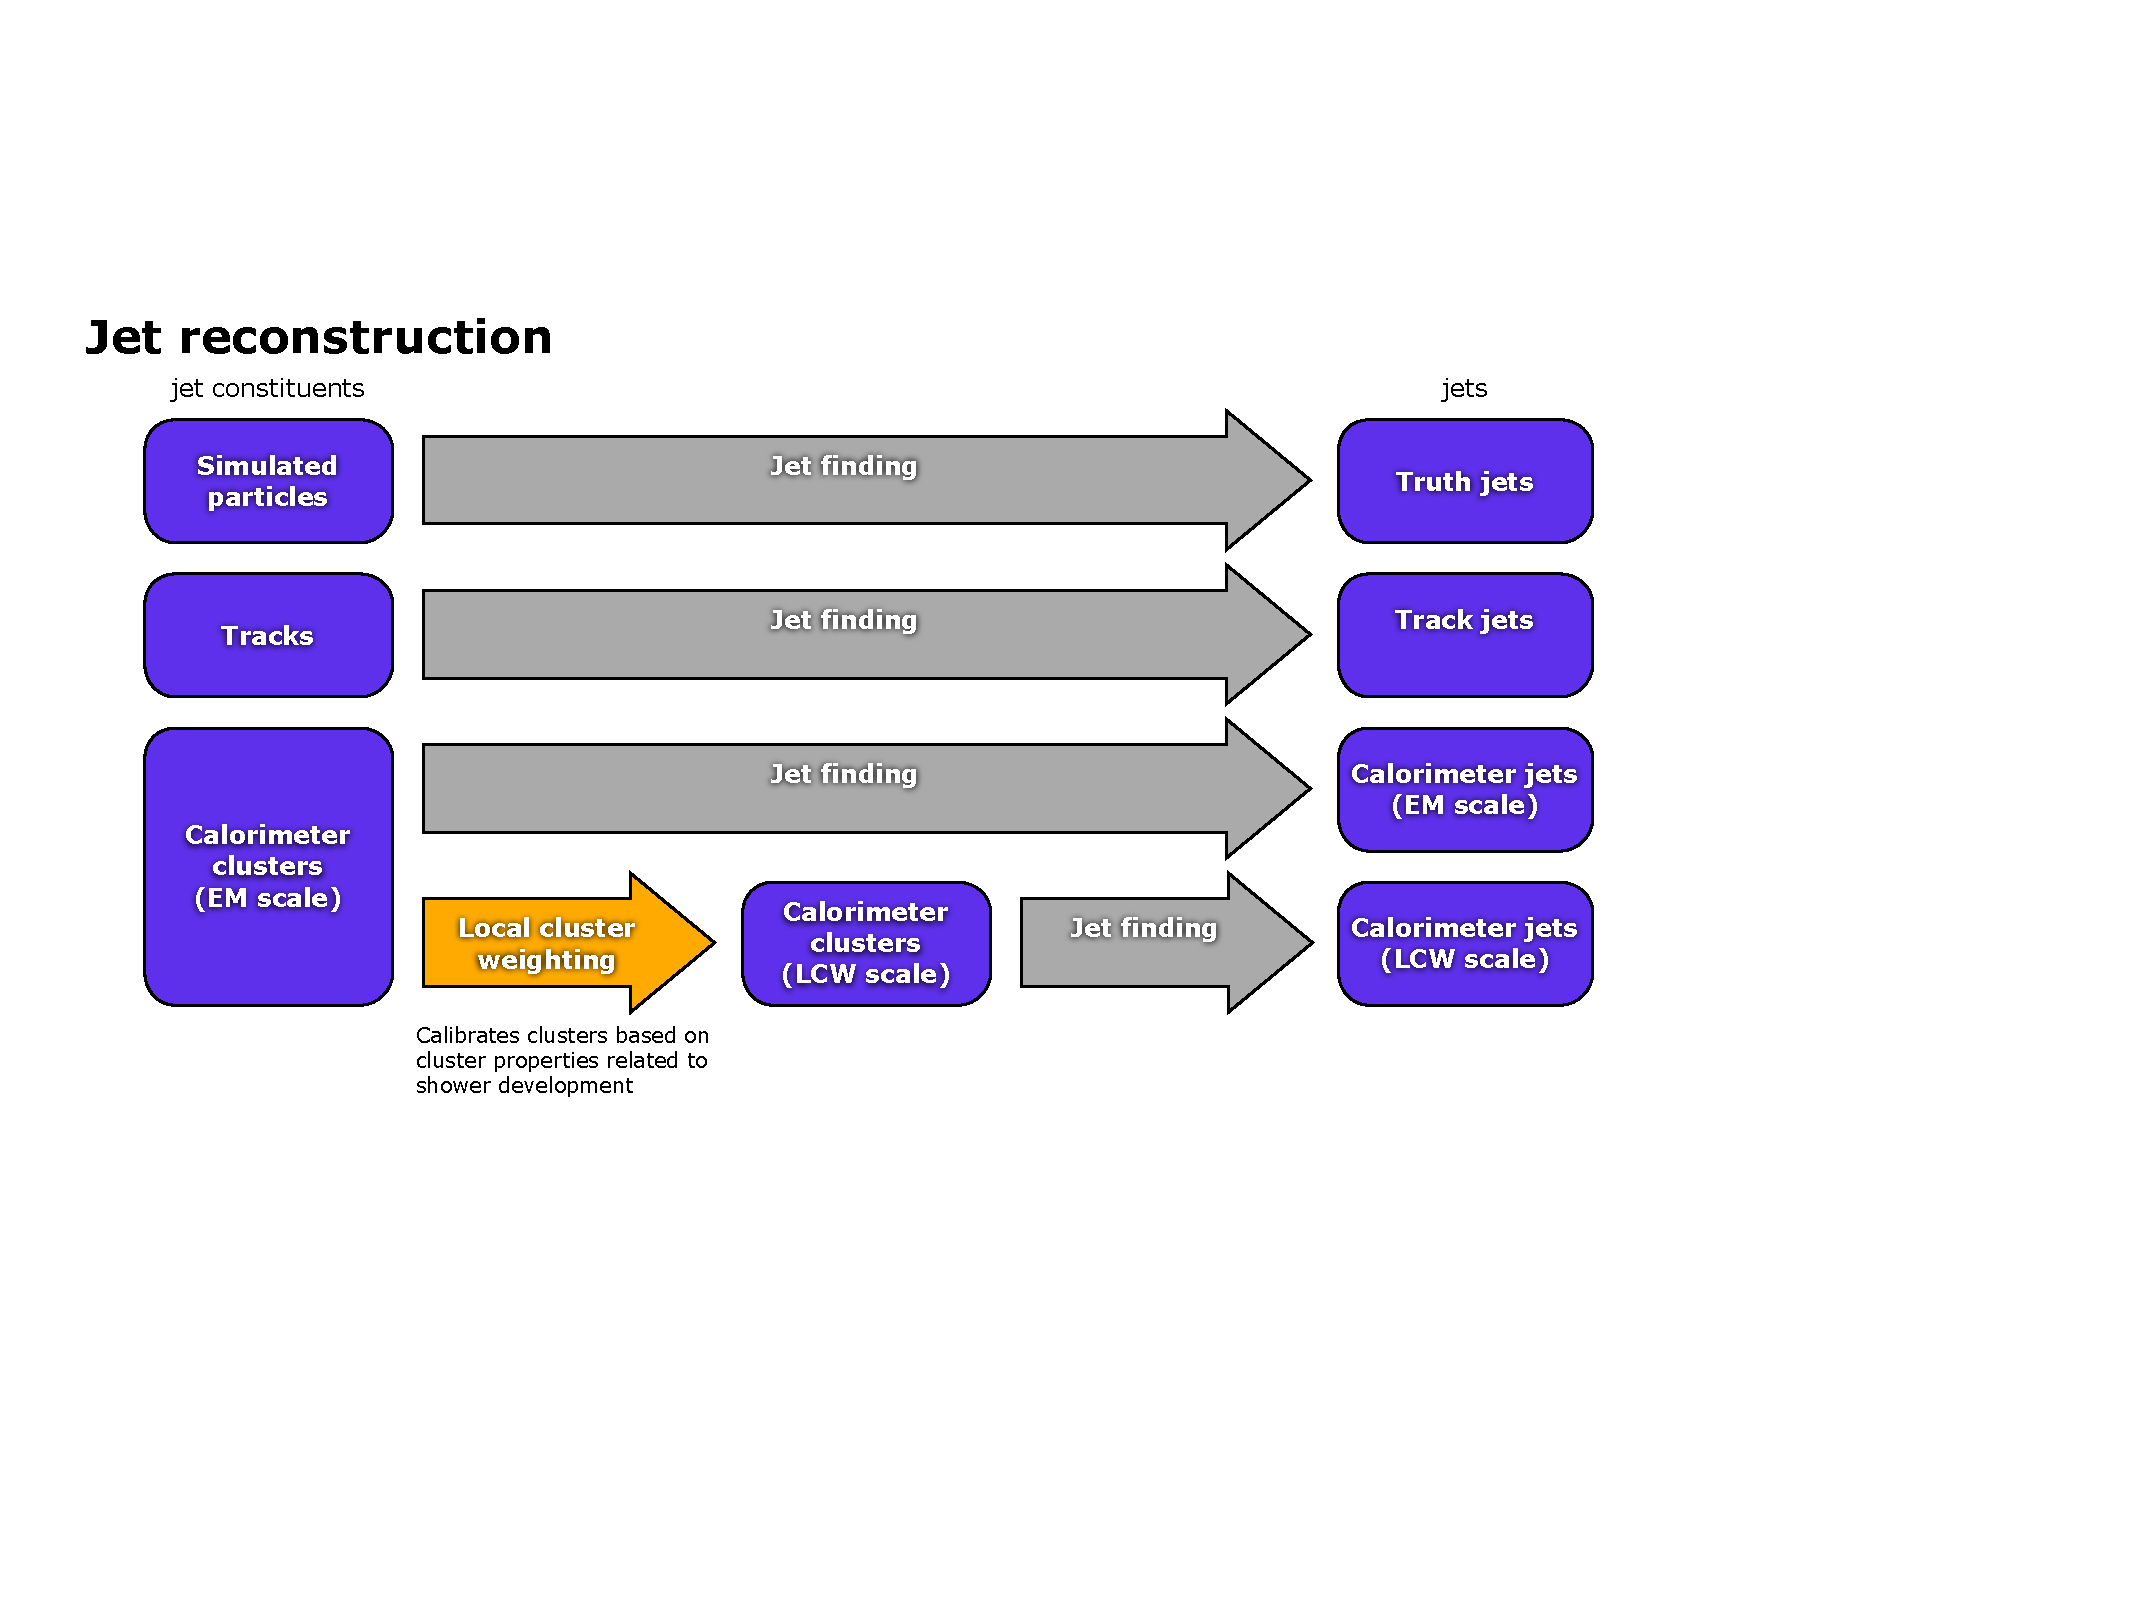
\includegraphics[width=0.7\textwidth]{making-jets.pdf}
\label{fig:jet-reconstruction:making-jets}
\caption{A diagram showing the various forms of jet inputs, and the different types of jets they are used to make.}
\end{figure}

%%%%%%%%%%%%%%%% 

Jets constructed from the simulated particles from a Monte Carlo generator are called \textit{truth jets}: these are primarily used to study the performance of algorithms without the effect of the detector, and to calibrate and define the resolution of other classes of jets. 

Jets can also be constructed from tracks, the outputs of pattern recognition algorithms performed on the hits in the Inner Detector, which correspond to the trajectories of charged particles. These \textit{track jets} are mostly used for validation: they provide a completely independent measurement of a jet from the calorimeter, and while they miss the neutral third of particles, the increased angular precision of tracking can result in complementary information to the calorimeter measurement. \editnote{Cite Seth's thesis, substructure paper?} 

Finally, and most importantly, jets can be formed from energy deposits left in the calorimeter, and these are called \textit{calorimeter jets}. Historically, ATLAS went through many different options for reducing the calorimeter information to a more manageable form for input to jet algorithms-- algorithms such as Global Cell Weighting, Noise Suppressed Towers, and simple projective towers were all eventually disfavored compared to the topo-clustering algorithm described in Section~\ref{jet-reconstruction:jet-inputs:topoclustering}. Calorimeter measurements all share several properties: they provide a measurement of the total energy of the parton shower, produced in both neutral and charged particles. This measurement of the jet (after relevant calibrations are applied) is at approximately the same scale as the quark which initiated it: for example, the invariant mass of the leading non-$b$-tagged jets in semi-leptonic $t\bar{t}$ peaks at the value of the mass of the $W$-boson, $m_{W} = 80$~GeV. Calorimeter jets can thus be used as 4-vectors in the same way that other detector objects-- electrons, photons, etc.-- are used (though of course there is more information in the structure of these jets, which analyses in this thesis do exploit).  \editnote{so many citations needed}

One alternative to separate tracking and calorimeter reconstructions of jets is to use a ``particle flow'' algorithm to combine the measurements from the separate detectors into coherent particle candidates which an be used as inputs to jet algorithms. Such algorithms exploit the fact that charged particles are much more accurately measured (up to some crossing point determined by the strength of the magnetic field) by tracking systems rather than calorimeter systems. Typically, tracks are extrapolated to the calorimeter and matched to energy deposits there; these matched deposits are then subtracted from the calorimeter, as the energy is already accounted for by the tracker. Unmatched energy deposits are assumed to have been created by photons or neutral hadrons, and remain in the list of inputs. Thus, the best features of tracker measurements (accurate energy resolution, and very good angular precision) and calorimeter measurements (capability of measuring neutral particles, good energy resolution at high energies) are combined. The CMS detector is particularly well suited to such reconstruction: the calorimeters are inside the 3.8 T magnetic field (nearly two times stronger than ATLAS), so energy deposits are more widely separated and track-to-calorimeter matching is less ambiguous. Since two thirds of the particles in the jet are reconstructed with tracks instead of calorimeter measurements, the reduced performance of the CMS hadronic calorimeters is also less important. However, as ATLAS has a weaker (and smaller, spatially) magnetic field, and compartively stronger hadronic calorimeters, the improvement from this approached is much diminished and ATLAS has thus far not used the particle flow algorithm for analyses. \editnote{cite cite cite}

The following subsections describe some details of the topoclustering and tracking algorithms which form the inputs to the jet algorithms in ATLAS. The design decisions in these algorithms-- and the strong performance they achieve in the face of difficult operating conditions-- are critical for the final results of hadronic analyses on ATLAS.

\subsection{Topoclustering}
\label{jet-reconstruction:jet-inputs:topoclustering}

\subsection{Tracking}

Discussion of bending, out of cone

\subsubsection{Ghost Association}

Alternative to independent track jets

\subsection{Cluster Calibration}
\section{Jet Calibration}

\section{Flavor Tagging}

\section{Quark/Gluon Discrimination}
	\subsection{Lots of subsections}
		...